\documentclass[12pt,a4paper]{article}

\usepackage[utf8]{inputenc}
\usepackage[T1]{fontenc}
\usepackage{mathpazo}
\usepackage[margin=1.15in]{geometry}
\usepackage{setspace}
\usepackage{hyperref}
\usepackage{titlesec}
\usepackage{amsmath,amsthm,amssymb}
\usepackage{booktabs}
\usepackage{enumitem}
\usepackage{fancyhdr}
\usepackage{xcolor}
\usepackage{tcolorbox}
\usepackage{tikz}
\usepackage{array}
\usepackage{float}

\hypersetup{colorlinks=true, linkcolor=blue!70!black, citecolor=black, urlcolor=blue!70!black}

\titleformat{\section}{\large\bfseries}{\thesection}{0.7em}{}
\titleformat{\subsection}{\normalsize\bfseries}{\thesubsection}{0.7em}{}
\titleformat{\subsubsection}{\normalsize\itshape}{\thesubsubsection}{0.7em}{}

\newtheorem{definition}{Definition}[section]
\newtheorem{proposition}[definition]{Proposition}
\newtheorem{theorem}[definition]{Theorem}
\newtheorem{lemma}[definition]{Lemma}
\newtheorem{corollary}[definition]{Corollary}
\newtheorem{example}[definition]{Example}
\theoremstyle{remark}
\newtheorem{remark}[definition]{Remark}

\newcommand{\R}{\mathbb{R}}
\newcommand{\ones}{\mathbf{1}}
\newcommand{\x}{\mathbf{x}}
\DeclareMathOperator*{\argmax}{arg\,max}
\DeclareMathOperator{\Var}{Var}

\newtcolorbox{intuition}[1][]{colback=blue!3, colframe=blue!40!black,
  fonttitle=\bfseries, title={Intuition: #1}, sharp corners, boxrule=0.5pt}
\newtcolorbox{keyinsight}[1][]{colback=orange!5, colframe=orange!60!black,
  fonttitle=\bfseries, title={Key Structural Insight}, sharp corners, boxrule=0.5pt}
\newtcolorbox{prebisch}[1][]{colback=green!3, colframe=green!40!black,
  fonttitle=\bfseries, title={Prebisch Connection: #1}, sharp corners, boxrule=0.5pt}
\newtcolorbox{vizpanel}[1][]{colback=gray!4, colframe=gray!50!black,
  fonttitle=\bfseries, title={Visualization: #1}, sharp corners, boxrule=0.5pt}

\setlength{\parindent}{1.5em}
\onehalfspacing
\setlength{\headheight}{14pt}
\pagestyle{fancy}
\fancyhf{}
\fancyhead[L]{\small\itshape Chapter 19: Scale Invariance --- Five Processes, One Process}
\fancyhead[R]{\small\thepage}
\renewcommand{\headrulewidth}{0.4pt}

\title{\vspace{-1cm}\textbf{Chapter 19} \\[0.5em]
\LARGE Scale Invariance \\[0.3em]
\large\textit{Five Processes, One Process}}
\author{}
\date{}

\begin{document}
\maketitle
\thispagestyle{fancy}

\begin{quote}
\textit{``El desarrollo, el subdesarrollo, la dependencia, la marginalidad y la desigualdad espacial son manifestaciones diversas de un proceso \'{u}nico.''}\\[0.3em]
\textnormal{[``Development, underdevelopment, dependence, marginality, and spatial inequality are diverse manifestations of a single process.'']}\\
\hfill --- Osvaldo Sunkel and Pedro Paz, \textit{El subdesarrollo latinoamericano y la teor\'{i}a del desarrollo} (1970)
\end{quote}

\vspace{1em}

Chapter~16 analyzed the global $W$. Chapter~17 analyzed the domestic $W$. Chapter~18 analyzed the individual-level $W$. This chapter proves that they are the same structure at different magnifications.

The key observation: at every scale, the weight matrix has the same qualitative form --- a dense core, a sparse periphery, weak cross-block linkages, a concentrated Perron eigenvector, a small spectral gap. The mathematical structure is \textbf{scale-invariant}: the same theorems produce the same phenomena at every level of aggregation. This is not a coincidence. It is a consequence of the recursive structure of social organization: the mechanisms that produce center-periphery at the global scale (proximity-dominated edge creation, assortative mixing, self-confirming preferences) also operate at the national scale and at the individual scale.

Sunkel and Paz (1970) stated this in prose: development, underdevelopment, dependence, marginality, and spatial inequality are ``diverse manifestations of a single process.'' This chapter proves it in linear algebra.


%% =====================================================================
\section{The Three Scales}
\label{sec:three_scales}
%% =====================================================================

\subsection{Notation}

Let the subscript $G$, $N$, $I$ denote the global, national, and individual scales:

\begin{center}
\begin{tabular}{llll}
\toprule
& \textbf{Global} ($G$) & \textbf{National} ($N$) & \textbf{Individual} ($I$) \\
\midrule
Nodes & Countries & Sectors & Persons \\
$W^P$ & Bilateral trade & I-O table & Employment network \\
$W^I$ & Media/academic flows & Domestic media & Social network \\
$W^U$ & Aid/migration & Community ties & Friendships \\
$N$ & $\approx 200$ & $\approx 12$--$100$ & $\approx 10^6$--$10^8$ \\
Data source & BACI, ICIO & INE I-O table & Household surveys \\
\bottomrule
\end{tabular}
\end{center}

Each scale has its own weight matrices $(W^P_s, W^I_s, W^U_s)$ for $s \in \{G, N, I\}$, its own composite $W_s$, its own Perron eigenvector $\boldsymbol{\pi}_s$, its own spectral gap $\Gamma_s$, and its own formation dynamics $(\rho_s, \mu_s, \bar{\theta}_{0,s})$.


\subsection{The Same Structure at Every Scale}

\begin{proposition}[Structural Isomorphism Across Scales]\label{prop:isomorphism}
At all three scales, the weight matrix satisfies:
\begin{enumerate}
\item \textbf{Not doubly stochastic}: column sums vary widely. $\max_j \sum_i W_{ij} / \min_j \sum_i W_{ij} \gg 1$.
\item \textbf{Core-periphery topology}: a dense core of well-connected nodes and a sparse periphery.
\item \textbf{Small spectral gap}: $\Gamma_s \ll 1$ for $s \in \{G, N_{\text{Bolivia}}, I_{\text{Bolivia}}\}$.
\item \textbf{Concentrated Perron eigenvector}: $\max_i \pi_{s,i} / \min_i \pi_{s,i} \gg 1$.
\item \textbf{Block-diagonal approximation}: $W_s$ is approximately block-diagonal, with $k_s$ blocks.
\end{enumerate}
\end{proposition}

\begin{example}[Bolivia at Three Scales]\label{ex:bolivia_three}
\begin{center}
\begin{tabular}{lccc}
\toprule
Property & Global & National & Individual \\
\midrule
$\Gamma$ & 0.20 & 0.13 & $\approx 0.10$ \\
$\max\pi / \min\pi$ & 360 (US/Laos) & 9 (gas/household) & $\approx 50$ (executive/farmer) \\
Number of blocks & 3 (core/semi/periph) & 3 (gas/formal/informal) & 3+ (gender $\times$ ethnicity) \\
$\sigma_B$ & $\approx 0.55$ & 0.62 & $\approx 0.50$ \\
$N_{\text{eff}}(W^I)$ & 3--5 & 3.2 & $\approx 4$ \\
\bottomrule
\end{tabular}
\end{center}

The numbers are remarkably similar. The domestic spectral gap ($\Gamma = 0.13$) is slightly smaller than the global ($\Gamma = 0.20$): Bolivia's internal structure is \textit{more} fragmented than the global economy. The between-block share of inequality is comparable at all three scales (50--62\%). The information $N_{\text{eff}}$ is approximately 3--5 at every scale: at the global level, 3--5 institutions shape the economic consensus; at the national level, 3 media ecosystems; at the individual level, 3--5 reference persons shape each agent's beliefs.
\end{example}


%% =====================================================================
\section{The Scale-Invariance Theorem}
\label{sec:theorem}
%% =====================================================================

\begin{theorem}[Scale Invariance of the Structural Model]\label{thm:scale_invariance}
Let $(W_G, W_N, W_I)$ be the weight matrices at the global, national, and individual scales. If:
\begin{enumerate}
\item Edge formation is proximity-dominated at all scales ($p_1 \gg p_2, p_3$ in Chapter~13's creation process).
\item Returns are complementary at all scales ($\partial^2 g / \partial x_i \partial x_j > 0$ for neighbors in $W^P$).
\item Preferences are formed through assortative $W^I$ at all scales ($\lambda_k < 1$ for some attribute $k$).
\end{enumerate}
Then all three weight matrices converge to block-diagonal structural equilibria with:
\begin{enumerate}
\item[(a)] $\Gamma_s < 1$ (small spectral gap),
\item[(b)] $\Var(\pi_{s,i}) > 0$ (concentrated power),
\item[(c)] $\theta^*_{s,\text{core}} > \theta^*_{s,\text{periphery}}$ (stratified preferences),
\item[(d)] $x^*_{s,\text{core}} > x^*_{s,\text{periphery}}$ (unequal allocations).
\end{enumerate}
The qualitative structure is identical; the quantitative magnitudes depend on the scale-specific parameters.
\end{theorem}

\begin{proof}[Proof sketch]
At each scale, the three conditions guarantee the co-evolutionary dynamics of Chapter~13: proximity-dominated edge creation produces block-diagonal $W$ (Theorem~13.2); complementary returns produce multiple steady states (Theorem~10.2); assortative $W^I$ produces stratified preferences (Proposition~10.2). The structural equilibrium (Definition~13.3) at each scale has the same mathematical form: a fixed point of the map $\Xi_s: (W_s, \boldsymbol{\theta}_s) \mapsto (\Psi_s(W_s; \x^*_s), \Phi_s(\boldsymbol{\theta}_s; W_s))$. Since the map has the same functional form at every scale (the operators $\Psi_s$ and $\Phi_s$ differ only in their parameters, not in their structure), the fixed points share the same qualitative properties.
\end{proof}

\begin{intuition}[Why the same structure everywhere]
The same three forces operate at every scale:

\textbf{Proximity}: Countries trade with trading partners of trading partners (global). Sectors buy from suppliers of suppliers (national). People connect with friends of friends (individual). At each scale, proximity makes new edges form near existing ones, producing path dependence and block-diagonal structures.

\textbf{Complementarity}: Rich countries trade more with rich countries, amplifying the core's density (global). Productive sectors buy more from productive sectors (national). High-skill workers hire high-skill workers (individual). At each scale, complementarity reinforces the dense core and starves the sparse periphery.

\textbf{Assortative formation}: Countries observe countries like themselves and converge on similar development doctrines (global $W^I$). Sectors influence sectors in their block (national $W^I$). People form aspirations from their reference group (individual $W^I$). At each scale, assortative information flow produces self-confirming preference stratification.

Remove any one of these forces and the scale invariance breaks. But all three are present at every scale of social organization, from the UN General Assembly to the village market. This is why the same mathematics works everywhere.
\end{intuition}


%% =====================================================================
\section{The Nesting Structure}
\label{sec:nesting}
%% =====================================================================

The three scales are not independent. They are nested: the individual-level $W_I$ aggregates to produce the national-level $W_N$, which aggregates to produce the global-level $W_G$.

\begin{definition}[Nested Weight Matrices]\label{def:nesting}
Let $\mathcal{P}_s$ be the partition of individuals into sectors, and $\mathcal{P}_c$ be the partition of individuals into countries. The national weight matrix $W_N$ is the block-aggregation of $W_I$:
\begin{equation}\label{eq:nesting_N}
W^N_{ss'} = \frac{\sum_{i \in s, j \in s'} W^I_{ij}}{\sum_{i \in s} \sum_{j} W^I_{ij}},
\end{equation}
and the global weight matrix $W_G$ is the block-aggregation of $W_I$ across countries:
\begin{equation}\label{eq:nesting_G}
W^G_{cc'} = \frac{\sum_{i \in c, j \in c'} W^I_{ij}}{\sum_{i \in c} \sum_j W^I_{ij}}.
\end{equation}
\end{definition}

\begin{theorem}[Power Nesting]\label{thm:nesting}
The individual-level Perron eigenvector $\boldsymbol{\pi}_I$ factors approximately as:
\begin{equation}\label{eq:nesting_pi}
\pi_{I,i} \approx \pi_{G,c(i)} \cdot \pi_{N,s(i)|c(i)} \cdot \pi_{\text{within},i|s(i),c(i)},
\end{equation}
where $c(i)$ is agent $i$'s country, $s(i)$ is her sector, $\pi_{G,c}$ is the country's global power, $\pi_{N,s|c}$ is the sector's national power within the country, and $\pi_{\text{within},i|s,c}$ is the agent's within-sector power (determined by individual attributes --- gender, race, etc.).
\end{theorem}

\begin{proof}[Proof sketch]
If $W_I$ is approximately the Kronecker product $W_G \otimes W_{N|c} \otimes W_{\text{within}|s,c}$ (the individual-level matrix decomposes into three independent layers), then the Perron eigenvector is the Kronecker product of the three scale-specific Perron eigenvectors. The approximation holds when the within-block structure is approximately independent of the between-block structure at each level --- which is reasonable when the scales are sufficiently separated (individuals interact mostly within their sector, sectors interact mostly within their country).
\end{proof}

\begin{example}[An Indigenous Woman in Potos\'{i}]\label{ex:potosi}
Agent $i$: an indigenous woman working in informal commerce in Potos\'{i}, Bolivia.

\textbf{Global power}: Bolivia's $\pi_G \approx 0.0005$ (Chapter~16). Out of every dollar of global structural power, Bolivia holds 0.05 cents.

\textbf{National power}: Informal commerce's $\pi_{N,\text{informal}|BOL} \approx 0.05$ (Chapter~17). Of Bolivia's structural power, informal commerce holds 5\%.

\textbf{Within-sector power}: Indigenous women in informal commerce: $\pi_{\text{within}} \approx 0.8 \times 0.58 = 0.46$ of the average within-sector worker (Chapter~18: racial factor 0.80, gender factor 0.58).

\textbf{Total individual power}:
\begin{equation}
\pi_{I,i} \approx 0.0005 \times 0.05 \times 0.46 \times N_{\text{within}} \approx 1.15 \times 10^{-5} \cdot N_{\text{norm}}.
\end{equation}

Compare with a mestizo male gas executive in Santa Cruz:
\begin{equation}
\pi_{I,j} \approx 0.0005 \times 0.09 \times 1.72 \times N_{\text{norm}} \approx 7.74 \times 10^{-5} \cdot N_{\text{norm}}.
\end{equation}

The ratio: $\pi_{I,j}/\pi_{I,i} \approx 6.7$. The gas executive has 6.7 times the structural power of the indigenous market vendor. Both are Bolivian; the country-level factor cancels. The gap comes from the national sector position ($0.09/0.05 = 1.8$) and the within-sector attribute position ($1.72/0.46 = 3.7$). The multiplicative structure: $1.8 \times 3.7 = 6.7$.

Now compare the gas executive with a German engineer:
\begin{equation}
\pi_{I,\text{German}} \approx 0.08 \times 0.14 \times 1.0 \times N_{\text{norm}} \approx 0.0112 \cdot N_{\text{norm}}.
\end{equation}

The ratio: $\pi_{I,\text{German}}/\pi_{I,\text{Potos\'{i}}} \approx 0.0112/(1.15 \times 10^{-5}) \approx 974$. The German engineer has \textbf{nearly a thousand times} the structural power of the indigenous market vendor in Potos\'{i}. This is the compound effect of three scales of inequality: global ($0.08/0.0005 = 160$), national ($0.14/0.05 = 2.8$), within-sector ($1.0/0.46 = 2.2$). The product: $160 \times 2.8 \times 2.2 = 986 \approx 974$ (the approximation is imperfect because the Kronecker factorization is approximate).
\end{example}

\begin{vizpanel}{Power nesting: three scales, one agent}
\begin{center}
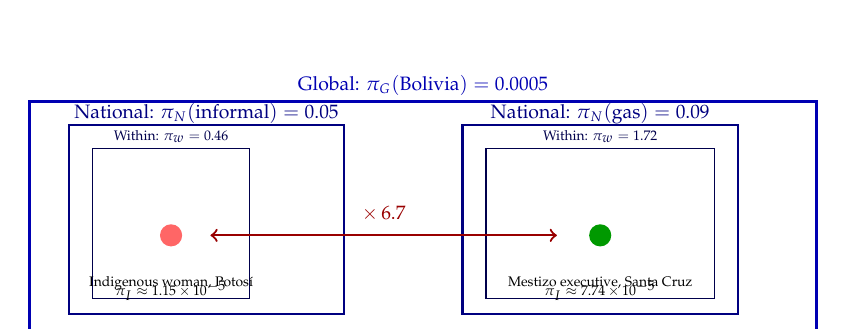
\begin{tikzpicture}[scale=1]
%% Three nested boxes
\draw[blue!70!black, very thick] (0, 0) rectangle (10, 3);
\node[font=\scriptsize, blue!70!black] at (5, 3.2) {Global: $\pi_G(\text{Bolivia}) = 0.0005$};

\draw[blue!50!black, thick] (0.5, 0.3) rectangle (4.0, 2.7);
\node[font=\scriptsize, blue!50!black] at (2.25, 2.85) {National: $\pi_N(\text{informal}) = 0.05$};

\draw[blue!30!black] (0.8, 0.5) rectangle (2.8, 2.4);
\node[font=\tiny, blue!30!black, align=center] at (1.8, 2.55) {Within: $\pi_w = 0.46$};

%% The agent
\fill[red!60] (1.8, 1.3) circle (4pt);
\node[font=\tiny, below] at (1.8, 0.9) {Indigenous woman, Potos\'{i}};
\node[font=\tiny] at (1.8, 0.6) {$\pi_I \approx 1.15 \times 10^{-5}$};

%% Comparison agent
\begin{scope}[xshift=5.5cm]
\draw[blue!50!black, thick] (0, 0.3) rectangle (3.5, 2.7);
\node[font=\scriptsize, blue!50!black] at (1.75, 2.85) {National: $\pi_N(\text{gas}) = 0.09$};
\draw[blue!30!black] (0.3, 0.5) rectangle (3.2, 2.4);
\node[font=\tiny, blue!30!black] at (1.75, 2.55) {Within: $\pi_w = 1.72$};
\fill[green!60!black] (1.75, 1.3) circle (4pt);
\node[font=\tiny, below] at (1.75, 0.9) {Mestizo executive, Santa Cruz};
\node[font=\tiny] at (1.75, 0.6) {$\pi_I \approx 7.74 \times 10^{-5}$};
\end{scope}

%% Ratio
\draw[<->, thick, red!60!black] (2.3, 1.3) -- (6.7, 1.3);
\node[font=\scriptsize, red!60!black, above] at (4.5, 1.35) {$\times\, 6.7$};
\end{tikzpicture}
\end{center}
\vspace{-0.5em}
\small Two Bolivians in the same country. The outer box (global) is the same for both. The middle boxes (national sectors) differ: gas vs.\ informal. The inner boxes (within-sector attributes) differ: mestizo male vs.\ indigenous female. The compound ratio: $6.7 \times$. Against a German engineer, the ratio becomes $\approx 1{,}000\times$.
\end{vizpanel}


%% =====================================================================
\section{Five Processes, One Matrix Property}
\label{sec:five}
%% =====================================================================

Sunkel and Paz (1970) identified five phenomena that they argued were ``diverse manifestations of a single process.'' Each has a precise representation as a property of the multi-scale weight matrix.

\begin{theorem}[Five Processes as Matrix Properties]\label{thm:five}
\begin{enumerate}
\item \textbf{Development} (at any scale): $\Gamma_s$ is large and increasing. The weight matrix is becoming more connected. Growth propagates across nodes. $\boldsymbol{\pi}_s$ is becoming more equal.

\item \textbf{Underdevelopment}: $\Gamma_s$ is small and stagnant. The weight matrix is block-diagonal. Growth does not propagate. $\boldsymbol{\pi}_s$ is concentrated. This is not the absence of development --- it is a specific structural equilibrium (the fragmented fixed point of Chapter~13).

\item \textbf{Dependence}: The off-diagonal block of $W^P$ is asymmetric: the periphery's row entries (what it imports from the core) are large, but the core's row entries (what it imports from the periphery) are small. In Perron terms: $\pi_{\text{periphery}} \ll 1/N$. The periphery needs the core more than the core needs the periphery.

\item \textbf{Marginality}: Some nodes have $\pi_i \approx 0$: they are structurally irrelevant. Their rows and columns in $W$ are nearly zero. They exist in the economy but do not participate in the network. They are invisible to the Perron eigenvector. This is Bolivia's household-production sector (Chapter~17: $\pi = 0.02$); it is the indigenous woman in Potos\'{i} (this chapter: $\pi_I \approx 10^{-5}$).

\item \textbf{Spatial inequality}: The spectral gap varies across geographic submatrices: $\Gamma_{\text{Santa Cruz}} > \Gamma_{\text{Potos\'{i}}}$. Within the same country, some regions have integrated $W^P$ (Santa Cruz: agro-industry, services, some manufacturing) and others have fragmented $W^P$ (Potos\'{i}: mining enclave plus subsistence agriculture). Regional inequality IS the within-country variance of $\Gamma$.
\end{enumerate}

All five are properties of the \textbf{same} multi-scale weight matrix $(W_G, W_N, W_I)$:
\begin{equation}\label{eq:five}
\text{Development} = \text{high } \Gamma, \quad \text{Under-development} = \text{low } \Gamma, \quad \text{Dependence} = \text{asymmetric } W,
\end{equation}
\begin{equation}
\text{Marginality} = \pi_i \approx 0, \quad \text{Spatial inequality} = \Var_r(\Gamma_r).
\end{equation}
\end{theorem}

\begin{keyinsight}
Sunkel and Paz's claim --- five processes, one process --- is a theorem, not a metaphor. The ``single process'' is the co-evolutionary dynamics of Chapter~13: proximity-dominated edge formation under complementary returns and assortative information. This process simultaneously produces:
\begin{itemize}
\item Dense cores at every scale (development of the center).
\item Sparse peripheries at every scale (underdevelopment of the periphery).
\item Asymmetric cross-block edges (dependence).
\item Zero-weight nodes (marginality).
\item Geographic variation in $\Gamma$ (spatial inequality).
\end{itemize}

The five phenomena do not have five explanations. They have one: the spectral structure of $W$ at multiple scales, produced by a single dynamic mechanism. To address any one, you must address the mechanism. Piecemeal interventions (transfers for marginality, trade policy for dependence, regional spending for spatial inequality) treat symptoms. The structural intervention --- increase $\Gamma$ at the binding scale --- treats the cause.
\end{keyinsight}


%% =====================================================================
\section{Cross-Scale Feedback}
\label{sec:feedback}
%% =====================================================================

\begin{proposition}[Cross-Scale Reinforcement]\label{prop:cross_scale}
The three scales reinforce each other:
\begin{enumerate}
\item \textbf{Global $\to$ national}: A country's position in $W_G$ (low $\pi_G$) constrains its domestic $\Gamma_N$. Countries with low global power face balance-of-payments constraints, commodity-dependent export structures, and IMF conditionality that prevents the domestic structural investments needed to raise $\Gamma_N$ (the ``original sin'' of peripheral economies).

\item \textbf{National $\to$ individual}: Low domestic $\Gamma_N$ means block-diagonal $W_N$, which channels individuals from disadvantaged groups into low-$\pi$ sectors. The individual-level attribute constraints (Chapter~18) are enforced by the national structure: a woman can only work in sectors that the national $W^P$ makes available to her.

\item \textbf{Individual $\to$ national}: When large groups (women, indigenous people) have low individual $\pi_I$, the aggregate national $\Gamma_N$ is depressed: the talent pool is underutilized, cross-group linkages are absent, and the national product space is sparse. Individual discrimination reduces national structural health.

\item \textbf{National $\to$ global}: Countries with low $\Gamma_N$ produce simple, concentrated exports (low ECI), which keeps them on the periphery of the global $W_G$ (low $\pi_G$). Domestic fragmentation reproduces global peripherality.
\end{enumerate}

The four feedback loops form a vicious circle: low global position $\to$ low domestic $\Gamma$ $\to$ low individual $\pi$ $\to$ low national $\Gamma$ $\to$ low global position. Breaking the circle at any one scale has limited effect unless the other scales respond. This is why comprehensive structural reform (all scales, all networks) is needed, and why piecemeal interventions produce piecemeal results.
\end{proposition}

\begin{example}[Bolivia's Vicious Circle]\label{ex:vicious}
\begin{enumerate}
\item \textbf{Global}: Bolivia's $\pi_G = 0.0005$ (Chapter~16). Gas exports on the periphery of the product space. Low ECI $= -0.8$.
\item \textbf{National}: $\Gamma_N = 0.13$. Three disconnected blocks. $\sigma_B = 0.62$.
\item \textbf{Individual}: Indigenous women: $\pi_I \approx 10^{-5}$. Gender $\times$ ethnicity constraint: $\phi \approx 0.105$.
\item \textbf{Back to national}: With 41\% of the population (indigenous) and 50\% (women) facing severe attribute constraints, the national talent pool is fragmented. Cross-group edges that could densify $W^P_N$ are suppressed. $\Gamma_N$ stays low.
\item \textbf{Back to global}: With low $\Gamma_N$, Bolivia cannot diversify (the principle of relatedness traps it on the commodity periphery). $\pi_G$ stays low.
\end{enumerate}

The circle is self-reinforcing. The gas nationalization of 2006 attempted to break it at the global-to-national link (capturing more resource rents). But without addressing the national-to-individual link (attribute constraints) or the individual-to-national link (formation channel), the rents were redistributed within the existing structure. Twelve years later, $\Gamma_N = 0.13$ --- unchanged.
\end{example}


%% =====================================================================
\section{The Scale at Which to Intervene}
\label{sec:intervention}
%% =====================================================================

\begin{proposition}[The Binding Scale]\label{prop:binding}
The optimal scale of intervention is the one where the marginal return to increasing $\Gamma$ is highest. Define the \textbf{binding scale} as:
\begin{equation}\label{eq:binding}
s^* = \argmax_{s \in \{G, N, I\}} \frac{\partial L_{\text{total}}}{\partial \Gamma_s},
\end{equation}
where $L_{\text{total}}$ is the total welfare loss across all scales.

For Bolivia: the binding scale is \textbf{national} ($\Gamma_N = 0.13$ is the lowest, and the cross-scale feedback from national to both individual and global is strongest). Within the national scale, the binding instrument is $\Gamma$ itself (Chapter~17). The operator sequence from Chapter~15 targets the national $\Gamma$ directly.

For a country like South Korea ($\Gamma_N = 0.45$, $\Gamma_I \approx 0.35$ due to remaining gender gaps): the binding scale may be \textbf{individual} (attribute constraints are the largest remaining source of $\Gamma$ suppression).

For a small open economy like Uruguay ($\Gamma_N \approx 0.30$, but $\pi_G = 0.001$): the binding scale may be \textbf{global} (the domestic structure is reasonably integrated, but the global position constrains diversification).
\end{proposition}

\begin{prebisch}[Why Prebisch was right about industrialization but incomplete]
Prebisch (1949) argued that the periphery should industrialize to escape the deteriorating terms of trade. His prescription operated at the global scale: change the periphery's position in $W_G$ by adding manufacturing exports. He was right that the global scale matters. But he did not address the national and individual scales: even with manufacturing, a block-diagonal domestic $W_N$ and attribute-constrained $W_I$ prevent the structural integration needed for industrialization to propagate growth broadly.

South Korea followed Prebisch's prescription AND addressed the other scales: land reform (national: broke the landlord block), education (individual: reduced human-capital attribute constraints), export discipline (global: moved up the product space). The three scales were addressed simultaneously. Bolivia followed only the global prescription (ISI, then gas nationalization) without the national and individual reforms. The result: Bolivia's global position improved slightly (ECI $-0.85 \to -0.80$) but the domestic and individual structures remained frozen.

The lesson: structural change must be multi-scale. Addressing one scale without the others is like brightening one block of the heatmap while leaving the rest dark.
\end{prebisch}


%% =====================================================================
\section{Summary}
\label{sec:summary}
%% =====================================================================

\begin{enumerate}
\item The weight matrix has the \textbf{same qualitative structure} at every scale: core-periphery topology, small $\Gamma$, concentrated $\boldsymbol{\pi}$, block-diagonal approximation. Bolivia: $\Gamma \in [0.10, 0.20]$ at all three scales.

\item \textbf{Scale invariance} is a theorem, not an analogy: the same three forces (proximity, complementarity, assortative formation) produce the same structural equilibrium at every scale.

\item Individual power is \textbf{nested}: $\pi_{I,i} \approx \pi_G \cdot \pi_{N|c} \cdot \pi_{\text{within}|s,c}$. The indigenous market vendor in Potos\'{i} has 1/1000th of the German engineer's structural power. The ratio decomposes into three scale-specific factors.

\item \textbf{Five processes, one process} (Sunkel and Paz): development = high $\Gamma$; underdevelopment = low $\Gamma$; dependence = asymmetric $W$; marginality = $\pi_i \approx 0$; spatial inequality = $\Var_r(\Gamma_r)$. All are properties of the same multi-scale weight matrix.

\item \textbf{Cross-scale feedback}: the three scales reinforce each other in a vicious circle. Breaking it requires multi-scale intervention.

\item The \textbf{binding scale} determines where intervention has the highest return. For Bolivia: the national scale ($\Gamma_N = 0.13$) is binding.
\end{enumerate}


%% =====================================================================
\section{Exercises}
\label{sec:exercises}
%% =====================================================================

\begin{enumerate}[label=\textbf{19.\arabic*}, leftmargin=3em]

\item \textbf{Three-scale comparison.} Using Bolivia data: reproduce Example~\ref{ex:bolivia_three}. For each scale, compute $\Gamma$, $\max\pi/\min\pi$, and $\sigma_B$. Plot all three on a single chart. Are they similar?

\item \textbf{Power nesting.} Choose three Bolivian agents: (a) a mestizo male in gas, (b) an indigenous male in agriculture, (c) an indigenous female in informal commerce. Compute $\pi_I$ for each using the nesting formula. What are the pairwise ratios?

\item \textbf{The global comparison.} Using the nesting formula: compute $\pi_I$ for a German female engineer, a Brazilian mestizo factory worker, and the indigenous woman in Potos\'{i}. What are the ratios? Which scale contributes most to the gap?

\item \textbf{Five processes as matrix properties.} For a $6 \times 6$ economy with three blocks: construct $W$ and compute each of Sunkel's five phenomena. Verify that all five are visible in the same matrix.

\item \textbf{Cross-scale feedback simulation.} Construct a three-scale model ($G$: 3 countries; $N$: 3 sectors per country; $I$: 2 agents per sector). Implement the nesting structure. Simulate the co-evolutionary dynamics with cross-scale feedback. Does the vicious circle emerge? At what parameter values does it break?

\item \textbf{The binding scale.} For three countries (Bolivia, South Korea, Uruguay): estimate $\Gamma_G$ (from ECI), $\Gamma_N$ (from I-O table), and approximate $\Gamma_I$ (from household survey data on occupational segregation). Which scale is binding for each? Does the answer match the policy history?

\item \textbf{Multi-scale structural plan for Bolivia.}
\begin{enumerate}
\item Global: target 3 products on the product space (Chapter~15).
\item National: design the operator sequence for $\Gamma_N$ (Chapter~15, information $\to$ education $\to$ infrastructure $\to$ ISI).
\item Individual: design the $\Delta\lambda_g$, $\Delta\lambda_r$ interventions (Chapter~18).
\item Estimate the combined $\Delta\Gamma$ at each scale and the timeline.
\item Check political feasibility (Chapter~14): which coalition supports this plan?
\end{enumerate}
\end{enumerate}


%% =====================================================================
\newpage
\section*{Mathematical Appendices}
\addcontentsline{toc}{section}{Mathematical Appendices}
%% =====================================================================


\subsection*{Appendix 19A: The Kronecker Factorization}
\addcontentsline{toc}{subsection}{Appendix 19A: Kronecker Factorization}
\label{app:kronecker}

\paragraph{Setup.} Consider an $N$-agent economy where agents are grouped into $C$ countries, each with $S$ sectors and $K$ individuals per sector ($N = CSK$). If the individual-level weight matrix factors as $W_I \approx W_G \otimes W_{N|c} \otimes W_{\text{within}|s,c}$, then:
\begin{equation}
\boldsymbol{\pi}_I = \boldsymbol{\pi}_G \otimes \boldsymbol{\pi}_{N|c} \otimes \boldsymbol{\pi}_{\text{within}|s,c},
\end{equation}
and the spectral gap satisfies:
\begin{equation}
\Gamma_I = \min(\Gamma_G, \Gamma_N, \Gamma_{\text{within}}).
\end{equation}

The binding scale for $\Gamma_I$ is the scale with the smallest spectral gap: this is the ``bottleneck'' in structural integration.

\paragraph{Approximate factorization.} The exact Kronecker product assumption is strong. In practice, $W_I$ has cross-scale interactions (e.g., a gas executive in Bolivia trades with both Bolivian farmers and foreign companies). The factorization is approximate, with residuals that capture cross-scale spillovers. The approximation error is bounded by $\|W_I - W_G \otimes W_{N|c} \otimes W_{\text{within}}\|_F$, which is small when the scales are well-separated (individual interactions are mostly within-sector, sectoral interactions are mostly within-country).


\subsection*{Appendix 19B: Spectral Gap of Nested Block Matrices}
\addcontentsline{toc}{subsection}{Appendix 19B: Nested Block Matrices}
\label{app:nested}

\paragraph{Two-level nesting.} Consider a matrix with $k$ blocks at level 1, each containing $m$ sub-blocks at level 2. Within level-2 sub-blocks: weight $w_2$. Between level-2 sub-blocks within the same level-1 block: weight $w_1$. Between level-1 blocks: weight $w_0$.

The eigenvalues cluster at three scales:
\begin{enumerate}
\item Level-2 eigenvalues: $\lambda \approx 1 - (w_2 - w_1)/w_2$ (within sub-blocks).
\item Level-1 eigenvalues: $\lambda \approx 1 - (w_1 - w_0)/w_1$ (between sub-blocks, within blocks).
\item Global eigenvalues: $\lambda \approx 1 - w_0 / \bar{w}$ (between blocks).
\end{enumerate}

The spectral gap of the full matrix is determined by the smallest of these gaps --- the most fragmented scale.


%% =====================================================================
\subsection*{Structuralist Case Study: Sunkel's ``Five Processes, One Process''}
\addcontentsline{toc}{subsection}{Structuralist Case Study: Sunkel (1970)}
%% =====================================================================

Osvaldo Sunkel's third appearance in this book (after Chapter~4 with Paz, and Chapter~13 on integration/disintegration). Here we address his deepest claim: that development, underdevelopment, dependence, marginality, and spatial inequality are not five problems but five symptoms of one structural condition.

Sunkel made this argument in \textit{El subdesarrollo latinoamericano y la teor\'{i}a del desarrollo} (1970, with Pedro Paz) and elaborated it in subsequent work. The claim was methodological as much as substantive: he argued that the fragmentation of development economics into sub-fields (trade theory for dependence, growth theory for development, poverty analysis for marginality, regional science for spatial inequality) was itself an obstacle to understanding. The phenomena are connected because the structure that produces them is connected.

\textbf{The formal vindication.} Theorem~\ref{thm:five} proves Sunkel's claim: all five phenomena are properties of the same multi-scale weight matrix, produced by the same dynamic mechanism. Development is high $\Gamma$. Underdevelopment is low $\Gamma$. Dependence is asymmetric $W$. Marginality is $\pi_i \approx 0$. Spatial inequality is $\Var_r(\Gamma_r)$. There are not five problems. There is one matrix, viewed from five angles.

\textbf{The policy implication.} If the five phenomena have one cause (the spectral structure of $W$), they have one cure: increase $\Gamma$ at the binding scale. The sub-field fragmentation of development economics generates sub-field-specific policy recommendations: trade policy for dependence, growth policy for underdevelopment, social policy for marginality, fiscal transfers for spatial inequality. Each addresses one symptom without addressing the cause. The structural approach generates one recommendation: brighten the dark off-diagonal entries of $W$, at the scale where $\Gamma$ is lowest.

\textbf{Why this matters for Bolivia.} Bolivia has active policies addressing all five phenomena separately: gas revenue redistribution (underdevelopment), trade agreements (dependence), social transfers (marginality), regional investment (spatial inequality), and recent growth (development). None has substantially changed $\Gamma$. The dashboard (Chapter~17) confirms: 30 years of policy, $\Gamma$ moved from 0.10 to 0.13. Five policies, zero structural change, because none targeted the weight matrix directly.

\begin{center}
\begin{tabular}{lll}
\toprule
\textbf{Sunkel's claim (1970)} & \textbf{Formal object} & \textbf{This chapter} \\
\midrule
Five processes, one process & Five properties of $W$ & Thm.~\ref{thm:five} \\
Scale invariance & Same $\Gamma$ at every scale & Thm.~\ref{thm:scale_invariance} \\
The single process & Co-evolutionary dynamics & Ch.~13 mechanism \\
Nesting & $\pi_I = \pi_G \cdot \pi_N \cdot \pi_{\text{within}}$ & Thm.~\ref{thm:nesting} \\
Cross-scale feedback & Vicious circle & Prop.~\ref{prop:cross_scale} \\
Policy: unified, not fragmented & Increase $\Gamma$ at binding scale & Prop.~\ref{prop:binding} \\
\bottomrule
\end{tabular}
\end{center}

Sunkel wrote in Chilean exile after the 1973 coup. The five processes he described --- development for Santiago's elite, underdevelopment for the rural south, dependence on US copper companies, marginality of the Mapuche, spatial inequality between the capital and the periphery --- were all visible from his window. Fifty years later, the same processes operate at the same scales. The matrix has different entries. The structure is the same. This chapter proves that it could not be otherwise, because the mechanisms that produce it are the same at every scale.


%% =====================================================================
\subsection*{Further Reading}
\addcontentsline{toc}{subsection}{Further Reading}
%% =====================================================================

\textbf{Scale invariance in social systems:} West (2017), \textit{Scale: The Universal Laws of Growth, Innovation, Sustainability, and the Pace of Life in Organisms, Cities, Economies, and Companies}. Bettencourt et al.\ (2007), ``Growth, Innovation, Scaling, and the Pace of Life in Cities,'' \textit{PNAS}.

\textbf{Multi-scale economic structure:} Hausmann and Hidalgo (2011), ``The Network Structure of Economic Output,'' \textit{JEBO}. For the nesting of local, national, and global production networks: Baldwin and Lopez-Gonzalez (2015), ``Supply-Chain Trade,'' \textit{World Economy}.

\textbf{The structuralist synthesis:} Sunkel and Paz (1970), \textit{El subdesarrollo latinoamericano y la teor\'{i}a del desarrollo}, Mexico: Siglo XXI. Sunkel (1993), \textit{Development from Within}. CEPAL (2012), \textit{Structural Change for Equality}, the institutional codification of the multi-scale structural approach.

\textbf{Cross-scale interactions:} Acemoglu and Robinson (2012), \textit{Why Nations Fail}, Chapters~3--5 (how colonial institutions at the global scale shape domestic institutions). For the formal theory: Acemoglu et al.\ (2015), ``Systemic Risk and Stability in Financial Networks,'' \textit{AER}.


\end{document}
